\documentclass{article}
\usepackage[margin=1.5in]{geometry}
\usepackage{amsfonts}
\usepackage{textcomp}
\usepackage{graphicx}
\usepackage{caption}
\usepackage{wrapfig}
\usepackage{amsmath}
\usepackage{tabto}
\usepackage{imakeidx}
\usepackage{titlesec}
\usepackage{filecontents}
\usepackage{url}
\usepackage{hyperref}
\usepackage{algorithm}
\usepackage{algorithmic}
\usepackage{amsmath}
\usepackage{amssymb}
\usepackage{dsfont}
\setcounter{secnumdepth}{4}


\title{\textbf{Image processing for extracting features}}
\author{Clément Chenevas-Paule, Alexandre Audibert}
\date{2020/2021}
\makeindex
\begin{document}
\setlength\parindent{0pt}

\begin{titlepage}
\maketitle
\end{titlepage}




\tableofcontents
\newpage


\section{Presentation of the problem}
\noindent
\subsection{Context}

Over the last fifteen years, thousands of people were killed by rockfalls incidents all
around the world. In January 1962, a total of 2,000 people died as a result of a landslide in
Peru, making this natural phenomenon an international disaster that needed to be overcome. Rockfalls are quantities of rock falling freely from a cliff face causing rock cuts for
highways and railways in mountainous areas. They result in disrupting road traffic in the
mountainous regions creating an unsafe environment for people. Climatic and biological
events are behind rockfalls: an increase in pore pressure due to rainfall infiltration, erosion
of surrounding material during heavy rain storms, chemical degradation, root growth or
leverage by roots moving in high winds are all in the panoply of environmental events
that results in rockfalls. There are many factors that affect the severity of a rockfall such
as the slope geometry, the surface material and its retarding capacity, the size and shape
of the rock, the coefficients of friction of the rock surfaces and many others. Their study
is therefore important as it allows us to define secure areas for building houses and roads

\subsection{Study from experinental outcomes and acquisition of images}

One of the way to study this rock falls is based one experimental trials done over
a simple scaled model that is supposed to mimic some possible geographical topography. All the trials were realized in laboratory and in various conditions (a combination
of the environmental conditions defines each setup of the experience). The experimental process is the following : a collection of n identical objects are throw from the top
of the slope and a photo is taken of the deposit area. The scaled model is built as follows :\\



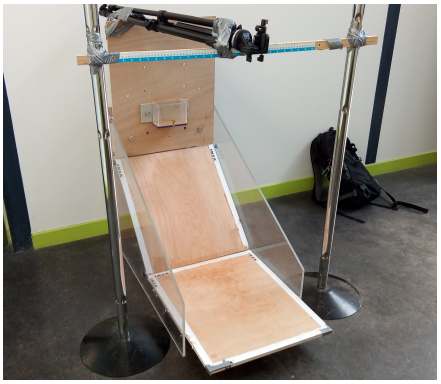
\includegraphics[width=5.5cm]{images/img1.png} 
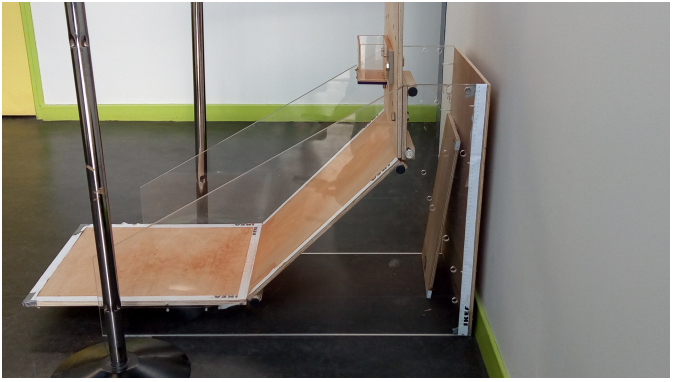
\includegraphics[width=8cm]{images/img2.png} 


\subsection{Image processing}

Up to now each photo was treated partially manually to produce a file where were collected the positions of thrown objects in a .csv file, and some other informations describing
the setup of the trial.
Each photo is treated with logiciel ImageJ and when clicking over each barycenter of
the objects the coordinates of each click are given. Up to now 20 differents setups where
tested and for each of them 50 launches were done so that there are 50 photos to be
treated in each setup. An exemple of a photo (file.jpg) and R-plot of the points given a
file.csv (where are collected coordinates of the brick’s centers) are given below :\\

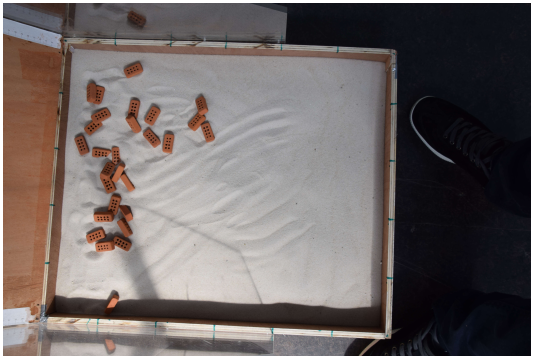
\includegraphics[width=6.8cm]{images/img3.png} 
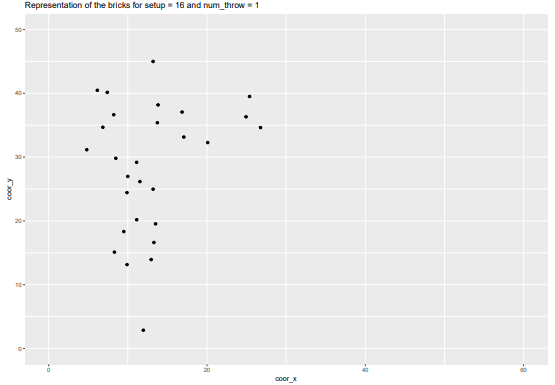
\includegraphics[width=6.8cm]{images/img4.png} 

The scaled model permits quite a lot of variations of the setup of the experimental
trials hence it becomes necessary to develop a completely automatic process for the treatment of each photo.

\subsection{Goal of this work and expected results}

Hence the main goal here is to built a tool that given a photo in format jpeg or
JPG will automatically produce a .csv file with coordinates of the objects stopped in the
deposit area.
In the following figures are shown the photo of one of the trials and the representation
of the the barycenter’s positions of the thrown objects that have arrived in the deposit
and photographied array.
Moreover it would be necessary to resize and adjust all the photos on the same rectangular pattern and possibly apply transformations to correct the parallax effects.
Some particular focus will be done over the situation where one brick is overponed on
another one. Even if some objects are mixed up it is also important to know how many
of them could be superimposed.

\subsection{Presentation of the report}

First of all, this report will present the main algorithms of image segmentation, edge detection, thresholding, ...\\
Secondly, this report will present how we use these famous algorithms to solve our problem. 

\section{Canny Edge Detection}



The Canny edge detector is an edge detection operator
The Process of Canny edge detection algorithm can be broken down to 5 different steps:

\begin{enumerate}
	\item Apply Gaussian filter to smooth the image in order to remove the noise
	\item Find the intensity gradients of the image
	\item Apply non-maximum suppression to get rid of spurious response to edge detection
	\item Apply double threshold to determine potential edges
	\item Track edge by hysteresis: Finalize the detection of edges by suppressing all the other edges that are weak and not connected to strong edges.
\end{enumerate}
\vspace{1 cm}

\subsection{Noice reduction by Gaussian filter}
Mathematical operation like gradient are really sensitive to noice on the image. Then the goal of this step is to delete noice in order to avoid false detection.

To reach this goal, the algorithm use a Gaussian filter. 
For that, we use a convolution between the image $I$ and a gaussian which takes in argumant $x$, $y$ and $\sigma$ :
 $$L(x , y , \sigma) = G(x , y , \sigma) * I (x , y )$$
where
 $$ G(x , y , \sigma) = \frac{1}{2\pi \sigma^2}exp(\frac{-(x^2+y^2)}{2\sigma^2}) \\$$
 with :\\
 - L is the smooth image.\\
 - The operator * is the convolution operator.\\
 - G is the gaussian smooth operator.\\
 - $x$ and $y$ are the coordinates.\\
 - $\sigma$ is the quantity of smooth. More $\sigma$ is big, more the smooth is big.\\
 - I is the picture.\\
\vspace{1 cm}

The convolution operator between an image and a kernel can be computed thanks to the next formula :
$$ g(x, y) = \omega * f(x, y) = \sum_{dx = -a}^a \sum_{dy = -b}^b \omega(dx, dy) f(x+dx, y+dy) $$
where $g(x,y)$ is the filtered image, $f(x,y)$ is the original image,$\omega$  is the filter kernel. Every element of the filter kernel is considered by $-a \leq dx \leq a$ and $-b \leq dy \leq b$.\\

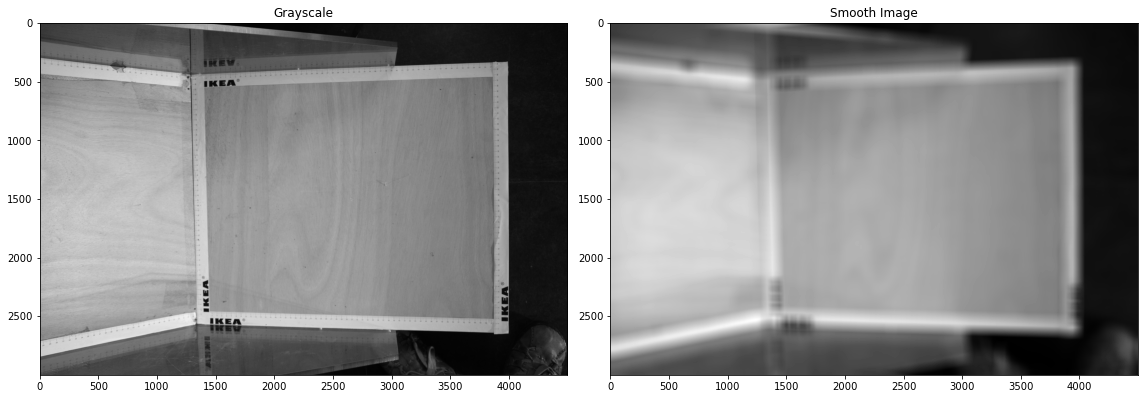
\includegraphics[width=14cm]{images/img5.png} 

We applied a gaussian filter of size $100$ with $\sigma = 1000$ on the left picture, the result appear on the right.\\
We volontary chose tremendous parameters to well visualize the effect of a gaussian filter but in reality we choose more reasonnable parameters.

\subsection{Finding the intensity gradient of the image}

Let's use a sobel filter to compute edge intensity and direction.
$$ K_x = \begin{bmatrix} -1 & 0 & 1 \\ -2 & 0 & 2 \\ -1 & 0 & 1 \end{bmatrix} , K_y = \begin{bmatrix} 1 & 2 & 1 \\ 0 & 0 & 0 \\ -1 & -2 & -1 \end{bmatrix} $$
$$ I_x = K_x * I $$
$$ I_y = K_y * I $$
The magnitude and the direction of the gradient is given by the formulas :
$$ |G| = \sqrt{I_x^2 + I_y^2} $$
$$ \theta(x, y) = atan2(I_y, I_x) $$
\vspace{1 cm}

These values are saved in $2$ matrices of the same size of the image.\\
Let's print the matrix of intensity as an image.\\

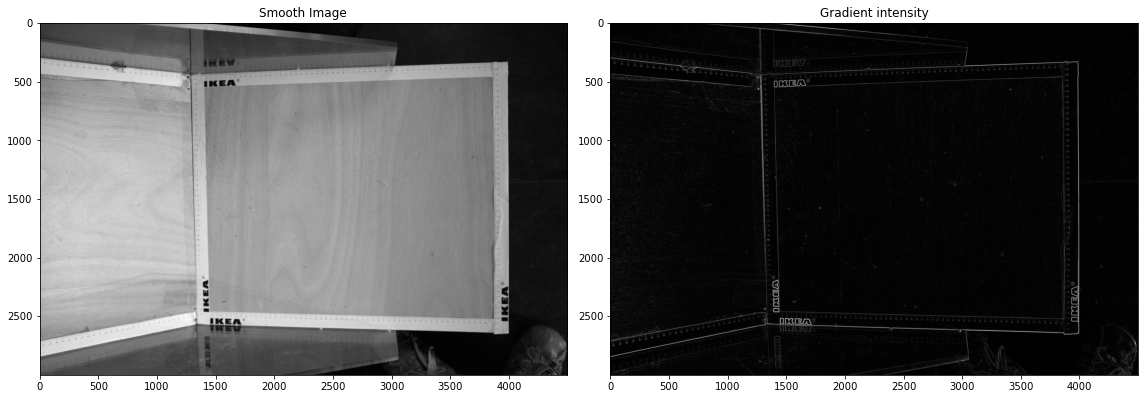
\includegraphics[width=14cm]{images/img6.png}

\subsection{Finding the intensity gradient of the image}

The gradient map obtained previously provides an intensity at each point of the image. A high intensity indicates a high probability of the presence of an outline. However, this intensity is not sufficient to decide whether a point corresponds to an outline or not. Only points corresponding to local maxima are considered to correspond to contours, and are retained for the next stage of detection.\\

The algorithm for each pixel in the gradient image is:\\
- Compare the edge strength of the current pixel with the edge strength of the pixel in the positive and negative gradient directions.\\
- If the edge strength of the current pixel is the largest compared to the other pixels in the mask with the same direction (e.g., a pixel that is pointing in the y-direction will be compared to the pixel above and below it in the vertical axis), the value will be preserved. Otherwise, the value will be suppressed.
\vspace{1 cm}


\begin{minipage}{.6\textwidth}%
In this example, we consider the pixel $(i, j)$.\\
Darker is the color of a pixel, greater is the intensity gradient.\\
The broken line represent the direction of the gradient of the considered pixel.\\
Toward this line, we can see that the pixel $(i, j)$ hasn't the biggest intensity, but the pixel $(i+1, j-1)$ has it.\\
As a result, we suppress the pixel $(i, j)$ because it is a non maximum.
\end{minipage}%
\hfill
\begin{minipage}{.35\textwidth}%
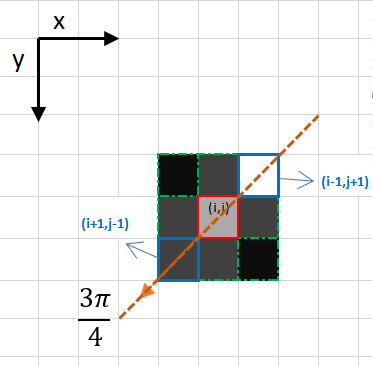
\includegraphics[width=\textwidth]{images/img7.png}
\end{minipage}%

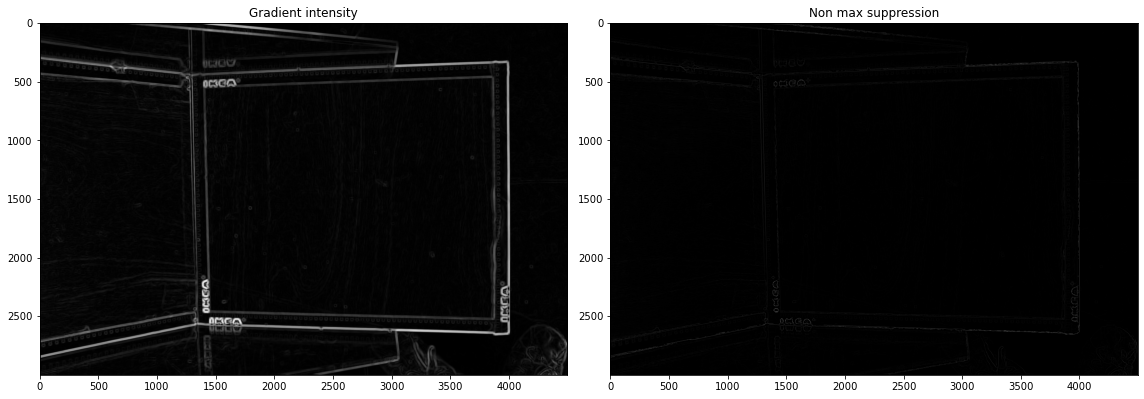
\includegraphics[width=14cm]{images/img8.png}
Here an application of the non maximum suppression on our image.

\subsection{Double threshold}

After application of non-maximum suppression, remaining edge pixels provide a more accurate representation of real edges in an image. However, some edge pixels remain that are caused by noise and color variation. In order to account for these spurious responses, it is essential to filter out edge pixels with a weak gradient value and preserve edge pixels with a high gradient value. This is accomplished by selecting high and low threshold values. If an edge pixel's gradient value is higher than the high threshold value, it is marked as a strong edge pixel and it is conserved. If an edge pixel's gradient value is smaller than the high threshold value and larger than the low threshold value, it is marked as a weak edge pixel. If an edge pixel's gradient value is smaller than the low threshold value, it will be suppressed. The two threshold values are empirically determined and their definition will depend on the content of a given input image.
\vspace{1 cm}

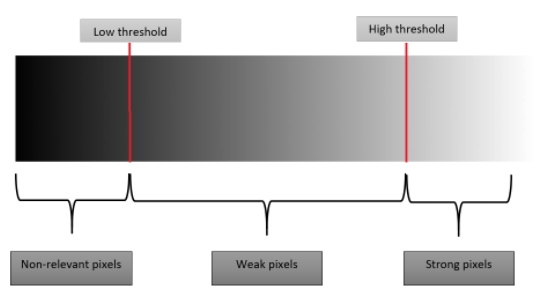
\includegraphics[width=12cm]{images/img9.png}

\subsection{Edge tracking by hysteresis}
Based on the threshold results, the hysteresis consists of transforming weak pixels into strong ones, if and only if at least one of the pixels around the one being processed is a strong one.
\vspace{1 cm}

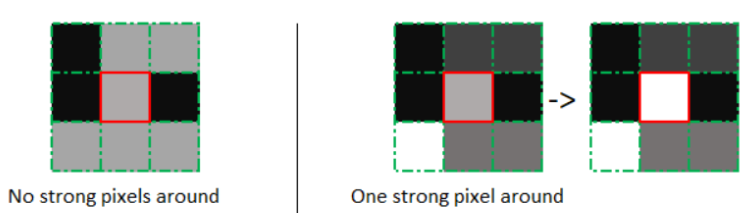
\includegraphics[width=12cm]{images/img10.png}

Here appear $2$ possible examples.\\
White represents strong pixels, black represents non relevant pixels and gray represents weak pixels. \\
On the left, the considered pixel (which is of course a weak pixel) has no strong pixel in his neighbourhood. As a result it turns to a non relevant pixel.\\
At the opposite, on the right example, a strong pixel belongs to the neighbourhood of the considered one so it turns to a strong pixel.\\

In our image this gives us :\\
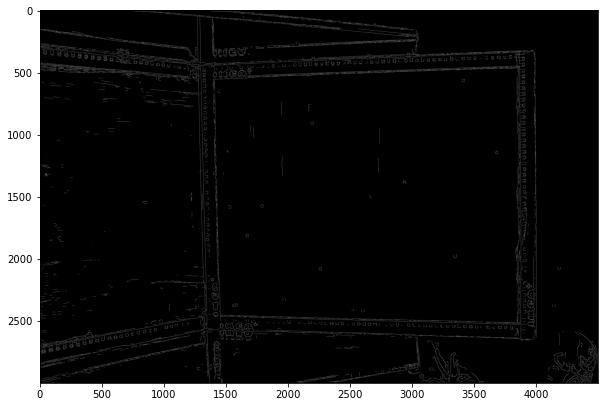
\includegraphics[width=12cm]{images/img11.png}

This picture is a binary image in which white pixels are considered to belong to a contour whereas black pixels don't belong to a contour.


\section{Hough transform}

The aim of the algorithm of Hough is to detect the lines of a picture, but it can also to detect circles or even other forms.

\subsection{Line detection}

\subsubsection{Hough space}

Classically, a line is represented by its equation $y = ax+b$ but if the line tends to the vertical, $a$ will tend to $+ \infty$. To avoid this problem, we represent a line thanks to its polar coordinates $\rho$ and $\theta$.

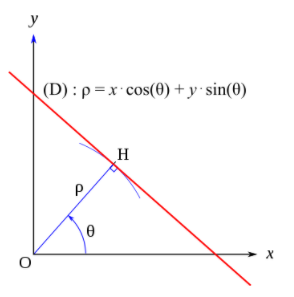
\includegraphics[width=7cm]{images/img17.png}\\
source : \url{https://fr.wikipedia.org/wiki/Transform%C3%A9e_de_Hough}\\

$\lbrace (\rho, \theta) \rbrace$ is then call Hough space.

In the Hough space, a line is obviously represented by a point and the set of all lines going through a given point is a sinusoidal curve.\\

\textbf{Demonstration :}\\
We fix $(x_0, y_0)$ a point in the cartesian plan. \\
We are searching for the collection of all the $(\rho, \theta)$ representing a line going through $(x_0, y_0)$.\\
$\rho = x_0.cos(\theta)+y_0.cos(\theta) \Rightarrow \rho = \sqrt{x_0^2 + y_0^2}(\dfrac{x_0}{\sqrt{x_0^2 + y_0^2}}.cos(\theta)+\dfrac{y_0}{\sqrt{x_0^2 + y_0^2}}.cos(\theta)) \Rightarrow \rho = \sqrt{x_0^2 + y_0^2}(cos(\phi)cos(\theta)+sin(\phi)sin(\theta)) \Rightarrow \rho = \sqrt{x_0^2 + y_0^2} cos(\theta - \phi)$\\
As a consequence,  the collection of all the $(\rho, \theta)$ representing a line going through $(x_0, y_0)$ is :\\
$\lbrace (\rho, \theta) \in \mathbb{R} \times [0, \pi] | \rho =  x_0.cos(\theta)+y_0.cos(\theta) \rbrace = \lbrace (\rho, \theta) \in \mathbb{R} \times [0, \pi] | \rho =  \sqrt{x_0^2 + y_0^2} cos(\theta - \phi) \rbrace$
which is a sinusoidal curve in the Hough space.\\


In the next example, red curve $A$ represents the set of all lines going through the blue point $A$. It is the same for $B$ and $C$.


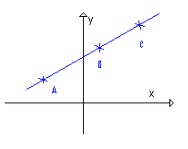
\includegraphics[width=6.8cm]{images/img18.png} 
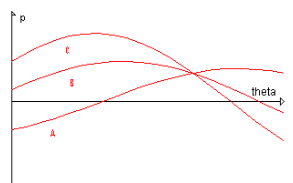
\includegraphics[width=6.8cm]{images/img19.png}\\
source : \url{https://fr.wikipedia.org/wiki/Transform%C3%A9e_de_Hough}\\

The 3 red lines cross in the same point, this point represents the unique line which going through $A$, $B$ and $C$.\\
We will use this principle in the Hough's algorithm.

\subsubsection{Hough alorithm}

We assume that a line of the image make part of a contour so the first step is to find a binary image with contours in white and other pixels in black. The Canny algorithm is well adapted for achieve this task, but other methods like gradient can be used.\\

The Hough's transform algorithm uses a 2-D matrix called accumulator. This accumalator is a discretisation of the Hough space.

\begin{algorithm}
\caption{Hough's algorithm}
\begin{algorithmic} 
\STATE $I \leftarrow $ image
\STATE $J \leftarrow $ contours of $I$ (by using Canny for instance)
\STATE $\delta \leftarrow $ discretisation step
\STATE $M \leftarrow $ accumulation matrix (discretisation of Hough space with step $\delta$)
\FOR{$(x, y) \in J$} 
\FOR{$\theta \in [0, \pi]$ with step $\delta$} 
\STATE $\rho = x.cos(\theta) + y.sin(\theta)$
\STATE $M[\rho, \theta] += 1$
\ENDFOR
\ENDFOR
\RETURN M
\end{algorithmic}
\end{algorithm}

Then we can represent the accumulator thanks to the next figure, more a point is white, bigger is its value in the accumulator.\\

In the next example, easily understand than this accumulator represents $2$ points in Hough space so the original image contains $2$ lines.\\

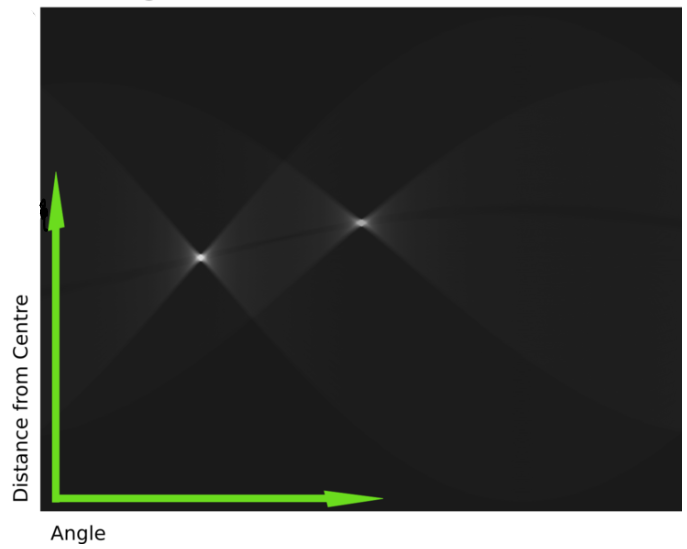
\includegraphics[width=8cm]{images/img20.png}\\
source : \url{https://en.wikipedia.org/wiki/Hough_transform} \\

In true images, the accumulator matrix is more complex than the previous one and we have to define hyperparameter which designs the threshold above which a point in the accumulator can be consider as a line in the original space.

\subsection{Circle detection}

We sow how we can use Hough algorithm to detect lines in an image. But in reality, we can use the same process for each form which can be represented by a finite number of parameters. This number of parameters is the dimension of our accumulator. \\
Let's take the example of circles.\\
We know that a circle can be reprensed by $3$ parameters. $a$ and $b$ such that $(a, b)$ is the center our the circle, and $r$ its radius. (Recall that the circle equation is $(x – a)^2 + (y – b)^2 = r^2$).\\
Then the process is the same but this time the accumulator is a discretisation of all the possible $a$, $b$ and $r$.
\newpage

\section{Homography}
In our case, we have many parallaxes problems. To solve this issue, Homography is used.
Example of parallaxe issu:
\begin{center}
    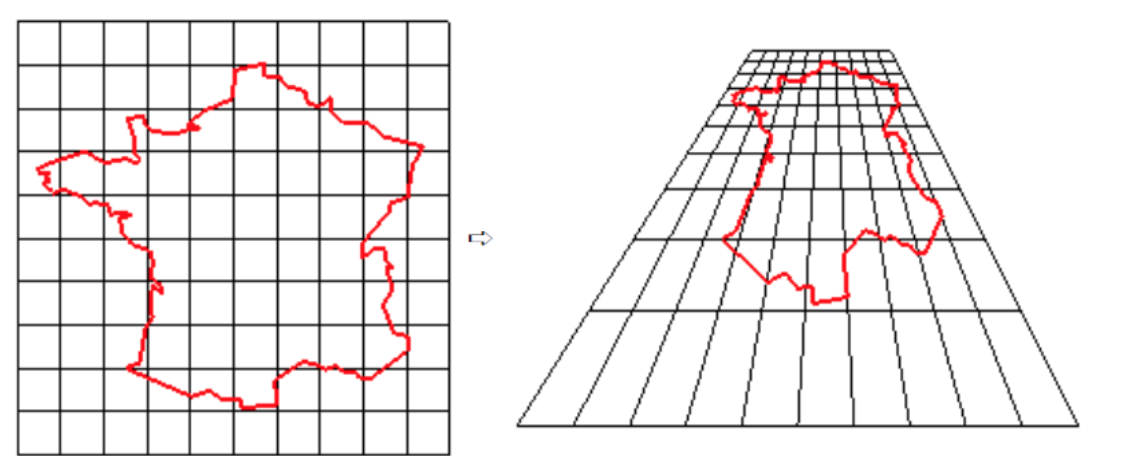
\includegraphics[scale=0.7]{images/parallax.png}    
\end{center}
\vspace{0.5 cm}

As reminder any two images of the same planar surface in space are related by a homography.We want to use this theory to return the tray to its original shape, i.e. a rectangle.
Before that It?s necessary to introduce an important mathematics notion, which is Homogenous coordinates.\\
This notion make it possible to characterise transformations in space with matrix.
Basically A point in cartesian coordinates, (X,Y) becomes  (X,Y,W)  in homogeneous coordinates.
\vspace{0.5 cm}

\begin{center}
    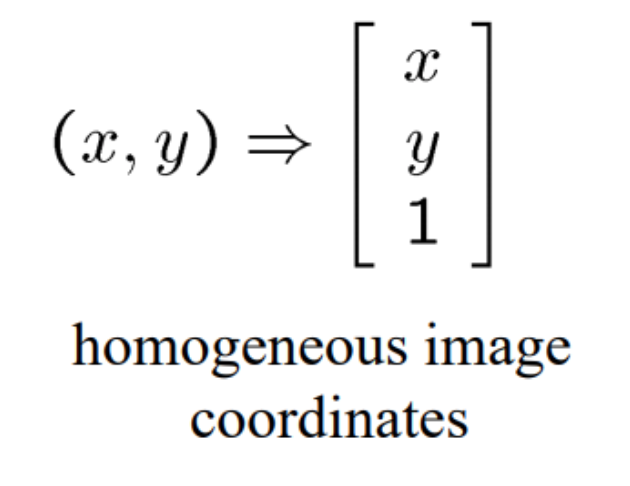
\includegraphics[scale=0.5]{images/homoge.png}  
    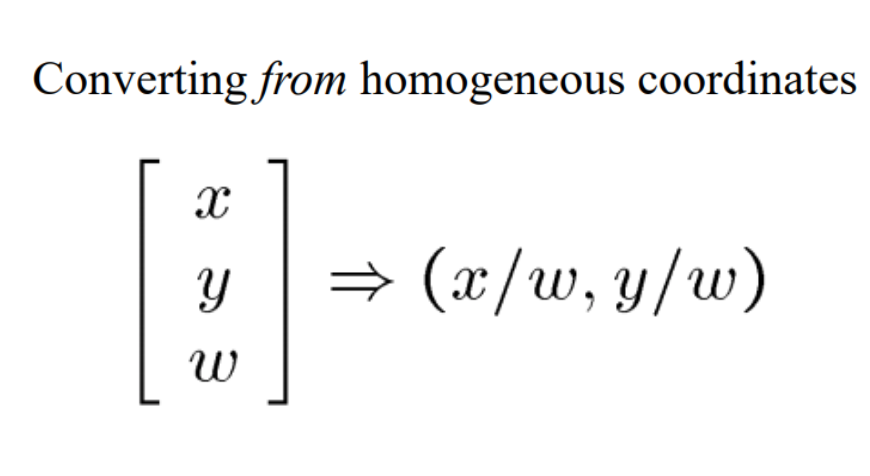
\includegraphics[scale=0.5]{images/homoge_2.png}      
\end{center}

In our case, transforming something like a parallelogram into a rectangle is called an affine transformation.  This transformation is obtained by applying the following matrix:
 $$H = \begin{bmatrix} a & b & c \\ d & e & f \\ g & h & 1 \end{bmatrix} $$.
 
 We want to find the matrix H such that for all pixels (x,y) in our picture where our tray is rectangular and ($x_0$,$y_0$) corresponding pixel to (x,y) in our original picture:
 $$\begin{bmatrix} a & b & c \\ d & e & f \\ g & h & 1 \end{bmatrix} \begin{bmatrix} x \\ y \\ 1 \end{bmatrix}  = \begin{bmatrix} x_0 \\ y_0 \\ z_0 \end{bmatrix}$$
 
 We can see that or equation depends on a new a paramter $z_0$. This parameter has a scaling role. The first step to find all pwith 
$$ x' = x_0 / z_0 $$
$$ y' = y_0 / z_0 $$

We can also write :
$$ z_0 \begin{bmatrix} x' \\ y' \\ 1 \end{bmatrix} = \begin{bmatrix} a & b & c \\ d & e & f \\ g & h & 1 \end{bmatrix} \begin{bmatrix} x \\ y \\ 1 \end{bmatrix} $$

By eliminating $c$ we can formulate the above equation in the form.
\begin{equation}
\left\lbrace
\begin{array}{ccc}
z_0 = gx + hy + 1 \\
x' \times z_0 = ax + by + c \\
y' \times z_0 = dx + ey + f
\end{array}\right.
\end{equation}

\begin{equation}
\left\lbrace
\begin{array}{ccc}
x' \times (gx + hy + 1) = ax + by + c \\
y' \times (gx + hy + 1) = dx + ey + f
\end{array}\right.
\end{equation}

\begin{equation}
\left\lbrace
\begin{array}{ccc}
ax + by + c  -  x'gx - x'hy - x' = 0\\
dx + ey + f - y'gx - y'hy - y' = 0
\end{array}\right.
\end{equation}

We get :

$$Ah = 0$$

with

$$ A = \begin{bmatrix} x & y & 1 & 0 & 0 & 0 & -x'x & -x'y & -x'  \\ 0 & 0 & 0 & x & y & 1 & -y'x & -y'y & -y' \end{bmatrix} $$
and
$$ h = \begin{bmatrix} a & b & c & d & e & f & g & h & 1  \end{bmatrix}^T $$

We can easily conclude that we have 8 unknown variables and if we know the correspondence between two pixels of the two images it gives us two equations. Basically we will use the 4 angles of the plate which are the easiest pixels to recognize.

To summary if you want to obtain our rectangular tray :\\
Note the function I(x,y) which takes as input the coordinates of a pixel of the target image and returns its colour. \\
Note the function I\textquoteright(x,y) which takes as input the coordinates of a pixel of the initial image and returns its colour.
\vspace{ 1 cm}

To calculate I(x,y):
We use the previous equation :
$$\begin{bmatrix} a & b & c \\ d & e & f \\ g & h & 1 \end{bmatrix} \begin{bmatrix} x \\ y \\ 1 \end{bmatrix}  = \begin{bmatrix} x_0 \\ y_0 \\ z_0 \end{bmatrix}$$
Finally we define I(x,y) like : I(x,y) = I\textquoteright($\frac{x_0}{z_0}, \frac{y_0}{z_0}$)
\vspace{1 cm}

\textbf{Some results}\\
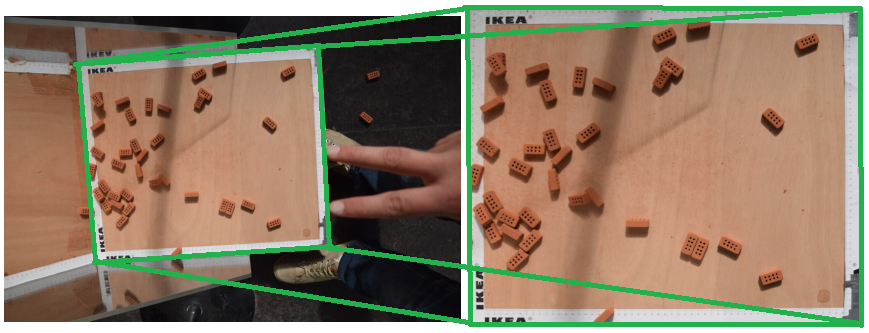
\includegraphics[width=12cm]{images/img21.png}


\section{Thresholding}

\subsection{Otsu method}
The OTSU method is used to perform automatic thresholding based on the shape of the image histogram.
This method applies to greyscale images and assumes that these images are composed of two classes which are the background and the objects.
This method has for goal to minimize the intra-class variance:\\
\\

First step is to create an Histogram function. The goal of hist(k) is to count the number of pixel equal to k. 
$$Hist(k) = \sum_{x,y} \mathds{1}_{I(x,y) = k} $$
Where I(x,y) is the intensity of pixel (x,y)

\vspace{0.5 cm}

The goal of our algorithm is to minimize the intra-class variance between our two classes.
Note the threshold : t

$$\sigma_w^2(t) = w_1(t)\sigma_1(t) + w_2(t)\sigma_2(t)$$
\\
where: 
\begin{itemize}
 \item $w_1(t) = \sum_{k = 0}^t \frac{Hist(k)}{N}$ probability to be in classe 1 and $w_2(t) = 1 - w1(t) $probability to be in classe 2
 \item $\sigma_i$ variance of class i.
\end{itemize}
\vspace{1 cm}
\textbf{Algorithm :}
\begin{enumerate}
\item  Calculate histogram function 
\item  for all possible t $\in \{0..255\}$ compute $\sigma_w^2(t)$ 
\item Find t which minimizes $\sigma_w^2(t)$ 
\item Transform or picture in binary image
\end{enumerate}
\vspace{1 cm}

\section{Morphological Transformations}

The first step of the morphological transformations is to define a kernel.\\
As an example, we will take a $5 \times 5$ sized kernel.
$$K = \begin{bmatrix} 1 & 1 & 1 & 1 & 1 \\ 1 & 1 & 1 & 1 & 1 \\1 & 1 & 1 & 1 & 1 \\1 & 1 & 1 & 1 & 1 \\1 & 1 & 1 & 1 & 1  \end{bmatrix}$$

\subsection{Erosion}

The erosion is used, as its name suggests, to erode an image like in the next example :\\


\includegraphics[width=6.8cm]{images/img12.png} 
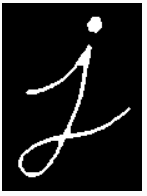
\includegraphics[width=6.8cm]{images/img13.png} \\
source : \url{https://opencv-python-tutroals.readthedocs.io/en/latest/py_tutorials/py_imgproc/py_morphological_ops/py_morphological_ops.html}\\

The kernel slides through the image (as in 2D convolution). A pixel in the original image (either 1 or 0) will be considered 1 only if all the pixels under the kernel is 1, otherwise it is eroded (made to zero).

\subsection{Dilatation}

At the opposite, dilatation dilate a image like in the next example :\\


\includegraphics[width=6.8cm]{images/img12.png} 

\includegraphics[width=6.8cm]{images/img14.png}\\ 
source : \url{https://opencv-python-tutroals.readthedocs.io/en/latest/py_tutorials/py_imgproc/py_morphological_ops/py_morphological_ops.html}\\

It is just opposite of erosion. Here, a pixel element is ‘1’ if at least one pixel under the kernel is ‘1’. So it increases the white region in the image or size of foreground object increases.

\subsection{Examples of use}

\subsubsection{Opening}

This operation consists in respectively execute an erosion, followed by a dilation. To goal of such an operation is to remove noise, as it appears on the next example :\\


\includegraphics[width=6.8cm]{images/img15.png} 

\includegraphics[width=6.3cm]{images/img16.png}\\
source : \url{https://opencv-python-tutroals.readthedocs.io/en/latest/py_tutorials/py_imgproc/py_morphological_ops/py_morphological_ops.html}\\


\section{Return to the problem}

Our problem is complex, because all the photos are really different. In fact, the point of view is never the same, the orientation of the trail can change, the luminosity also.\\
This is for instance visible in the next photos :\\
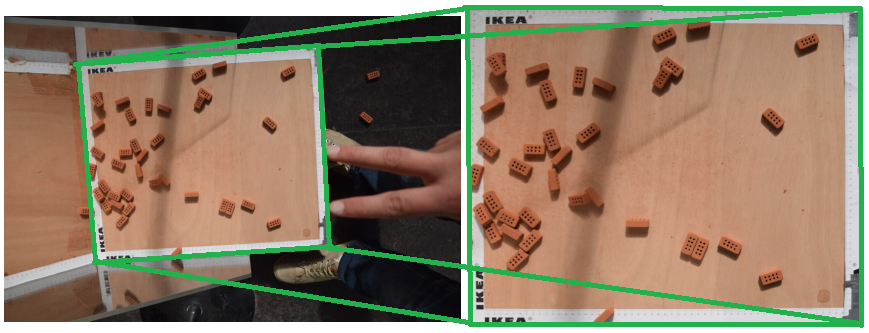
\includegraphics[width=6.8cm]{images/img21.jpg} 
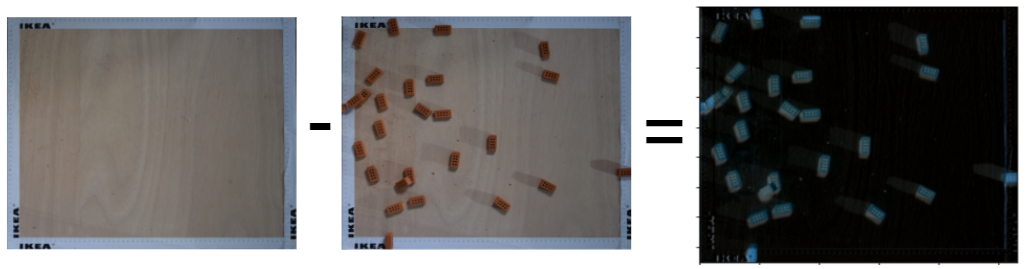
\includegraphics[width=6.8cm]{images/img22.jpg}\\
Thus we decide to cut the project in $2$ main parts :\\
 - The first part consists in searching for the $4$ sides of the trail (or the $4$ angulars, it is the same) and then apply an homography to extract the trail and suppress the projective effect of the photo.\\
 - The second part consists in searching for the position of the blocks in the extracted trail. Many strategies are tested and described in the next.

\subsection{Trail extraction}

\subsection{Blocks detection}

In this section, we suppose that for a given photo, we know the $4$ angulars of the trail.

The first step consists in doing an homography to extract the trail and suppress the projective effect. An example is given below.

\begin{center}
    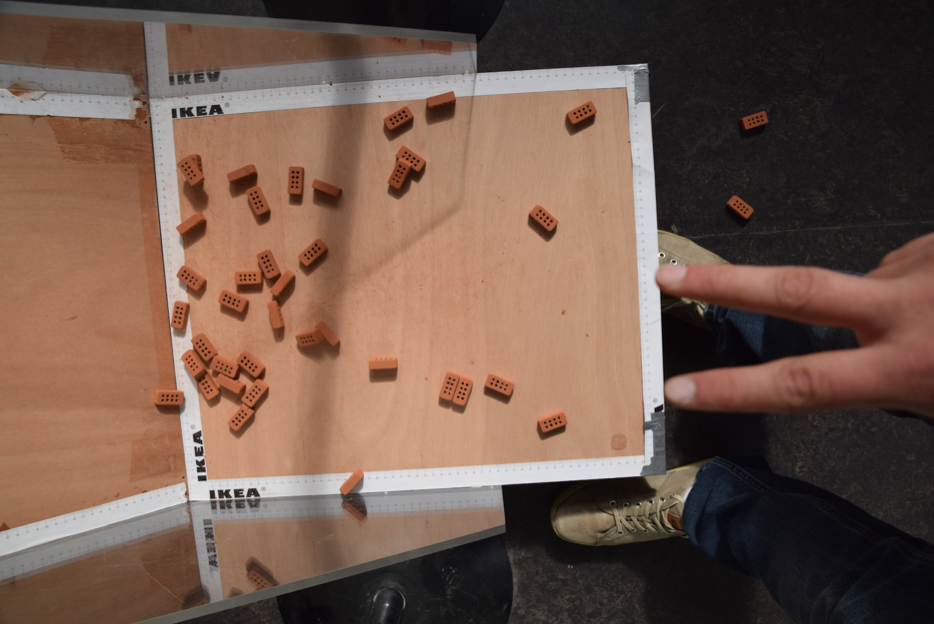
\includegraphics[scale=0.4]{images/result_1.png}  
    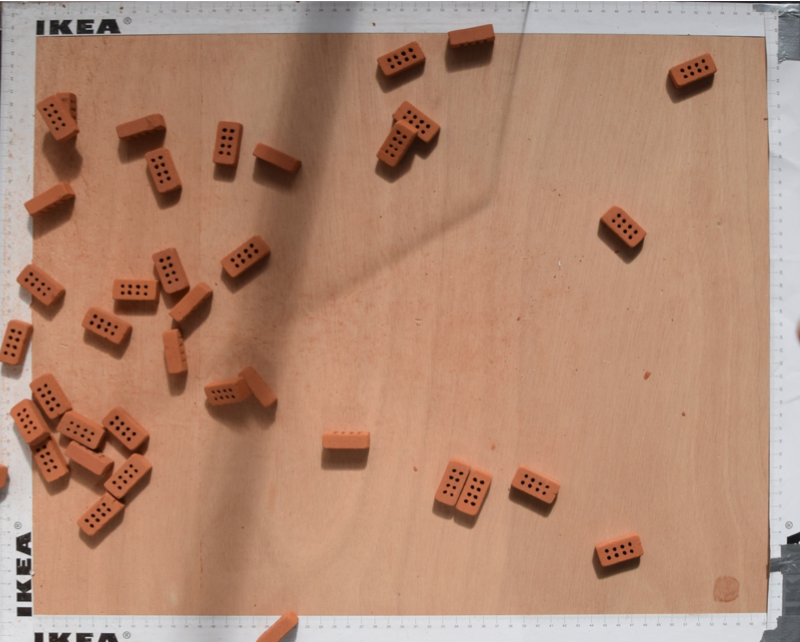
\includegraphics[scale=0.4]{images/resul_1.png}      
\end{center}

The work is now to use the right picture to find and extract the blocks.\\
Many strategies can be considered, we will have a look onthe mains ones we implemented.

\subsubsection{Strategy 1 : Watershed segmentation}

TO DO

\subsubsection{Strategy 2 : Threshold and Contours}

The first step of this strategy is simply a thresholding. The goal is to get an image similar to the next one :\\
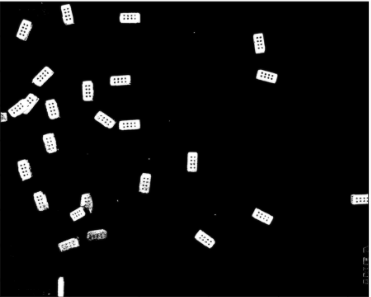
\includegraphics[width=7cm]{images/img23.png} \\
To reach susch a threshold, we can simlpy use a color threshold. This threshold is particularly efficient when the trail is well illuminated, whitout shadow and with blocks of color different from the floor.\\
Another mean to have such a threhold is to use the Otsu algorithm described earlier in this report.\\

\textbf{Important remark}.\\
In some case, we dispose of a photo of the trail before the rocks fall. This image can exploted in the same manner than the previous photos. That is to say that we can extract the trail, this will be particularly usefull as we will see soon.\\

One idea that we can exploit is to substract the empty trail with the full one. This give us the next result :\\ 

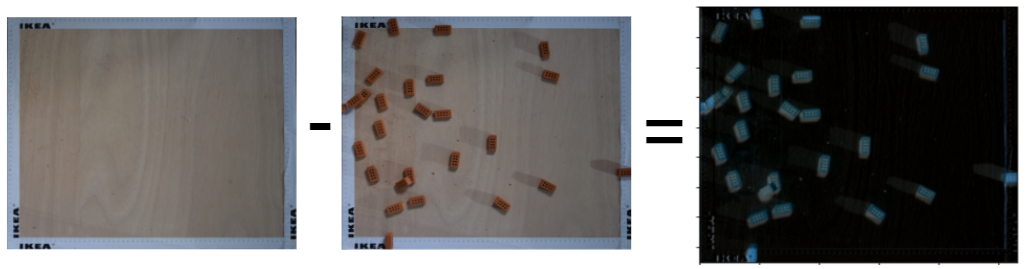
\includegraphics[width=14cm]{images/img22.png} \\
This operation is particularly interesting because it delete the white band, and other default of the image like the 'IKEA' written on the angular.\\
The threshold method are now more efficient because with have in the final image $2$ main colors.\\

For instance, an Otsu threshold on the previous image will give :\\
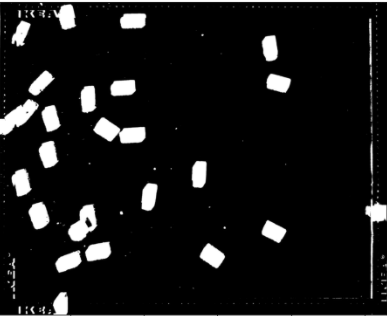
\includegraphics[width=7cm]{images/img24.png}\\

However, you can constat that some defaults exist on the image. These defaults are due to little movements of the camera (in the case of the photo substraction) or threshold errors otherwise.\\

This issue is easily solved thanks to an opening operation (see morphological transformations before).
If we apply succesively an erosin and a dilation on our image, we get :\\
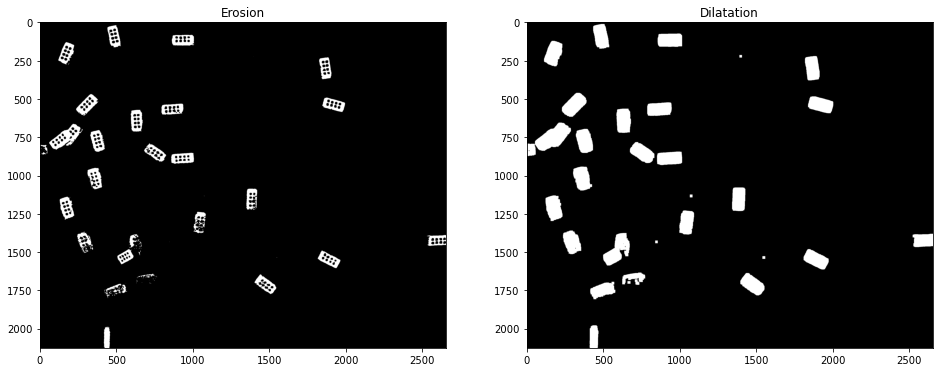
\includegraphics[width=14cm]{images/img25.png}\\ 


\subsubsection{Strategy 3 : Connex conponents}

To do

\section{Python Application}

To do : explain the fonctionality of the python app

\end{document}